\documentclass[12pt]{standalone}
\usepackage[utf8]{inputenc}
\usepackage{tikz}
\usetikzlibrary{arrows.meta}
\usepackage{graphicx}

\newcommand\smallSand{\tikz\draw[thick](0,0)circle(1.0);}
\newcommand\smallSlope{\tikz\draw[thick](-1,-1)--(-1,1)--(1,1)--(1,-1)--(-1,-1)--(-1,-0.25)--(1,0.25);}

\newcommand\bigSand{\tikz\draw[thick](0,0)circle(1.5);}
\newcommand\bigSlope{\tikz\draw[thick](-1,-1)--(-1,1)--(1,1)--(1,-1)--(-1,-1)--(1,1);}

\begin{document} 
   \begin{tikzpicture}[font=\sffamily]
		\node[inner sep=0pt] (fig) at (0,0) {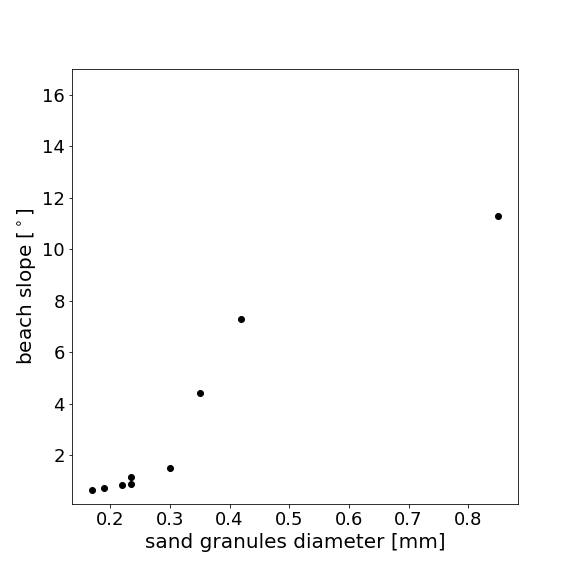
\includegraphics[]{plot1.png}};
		
		\node (smallSand) at (12,4.5) {\smallSand};
		\node (smallSlope) at (16,4.5) {\smallSlope};
		\draw[-{Latex[length=3mm]}](smallSand)--(smallSlope);
		
		\node (bigSand) at (12,0) {\bigSand};
		\node (bigSlope) at (16,0) {\bigSlope};
		\draw[-{Latex[length=3mm]}](bigSand)--(bigSlope);
		
		\node at (12,-4.5) {\huge{sand}};
		\node at (16,-4.5) {\huge{slope}};
   \end{tikzpicture}
\end{document} 